\section{Solution}\label{sec:solution}

In this part, we present our preliminary solution for achieving fast deadlock-free routing reconfiguration.

\subsection{Configuration Dependency Graph}\label{subsec:cdg}

\begin{figure}[t]
	\centering
	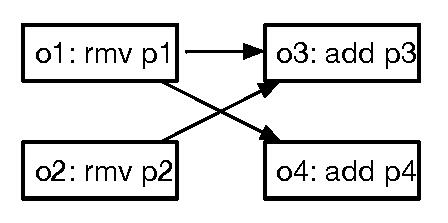
\includegraphics[width=0.45\textwidth] {figs/formulation_example}
	\caption{An example of configuration dependency graph.}\label{fig:cdgraph}
\end{figure}

In order to guarantee deadlock-free routing reconfiguration, we need to add some constraints to the executing order of path configuration operations. In this part, we define \textit{configuration dependency graph} (CDG) for the purpose of better describling the order constraints among different configuration operations.

CDG is a directed graph $G_c(V_c,E_c)$, where $V_c$ is a set of configuration operations, and $E_c$ is a set of order dependencies. Fig.~\ref{fig:cdgraph} shows an example of CDG. In the graph, each node represents a configuration operation. For example, node $o1$ represents the operation to remove path $p1$, while node $o3$ represents the operation to add path $p3$. Each directed edge in the graph represents an order constraint on the operations. For example,  $o1$ must be finished before we start the operation $o4$.

Let $P_c$ be the set of configuration paths in $G_c$. In Fig.~\ref{fig:cdgraph}, there are three legal configuration paths: 1) o1-o3; 2) o1-o4; 3) o2-o3. 

We use $ts(G_c)$ to denote a topological sorting of $G_c$. $ts(G_c)$ represents a possible order of configuration operations in terms of the finish time.  $TS(G_c)$ is the set of all possible topological sortings in $G_c$. In Fig.~\ref{fig:cdgraph}, there are five possible topological sortings: (o1, o2, o3, o4), (o1, o2, o4, o3), (o1, o4, o2, o3), (o2, o1, o4, o3) and (o2, o1, o3, o4). $P^{(i)}(ts)$ is  the set of active routing paths after first i-th operations in $ts(G_c)$ is finished. 

\subsection{Problem Formulation}\label{subsec:formulation}

\begin{table}
\begin{tabularx}{0.48\textwidth}{ |c||X| } 
	\hline
	$G(V,E)$ & The DCN, where $V$ is the set of all nodes and $E$ is the set of all links. \\ 
	\hline
	$C$ & $C \subset G(V,E)$ is a cycle in $G(V,E)$. \\ 
	\hline
	$P_s$ & The set of paths in the old configuration. \\
	\hline
	$P_t$ & The set of paths in the new configuration. \\
	\hline
%	$R_s$ & The set of rules corresponding to $P_s$. \\
%	\hline
%	$R_t$ & The set of rules corresponding to $P_t$. \\
%	\hline
%	$V_p$ & The set of nodes on path p. \\
%	\hline
%	$E_p$ & The set of links on path p. \\
%	\hline
	$R_p$ & The set of rules corresponding to path p. \\
	\hline

	$G_c(V_c,E_c)$ & A configuration dependency graph, where $V_c$ is a set of configuration operations, and $E_c$ is a set of order dependencies.\\
	\hline
	$P_c$ & The set of configuration paths in $G_c$.\\
	\hline
%	$t_o$ & The time to finish an operation $ o \in V_c$.\\
%	\hline
	$t(P, G_c)$& The time to configure all paths in $P$ obeying the dependencies in $G_c$.\\
	\hline
	$ts(G_c)$ & A topological sorting of $G_c$, which is a list of configuration operations. \\ 
	\hline
	$TS(G_c)$ & The set of all possible $ts(G_c)$. \\
	\hline
	$P^{(i)}(ts)$& The set of active paths after finishing first i-th operations in $ts(G_c)$.\\
	\hline
%	$P_s^{(i)}(ts)$& The set of remaining paths in $P_s$ after finishing first i-th operations in $ts(G_c)$.\\
%	\hline
%	$P_t^{(i)}(ts)$& The set of activated paths in $P_t$ after finishing first i-th operations in $ts(G_c)$.\\
%	\hline
	$d_{lx,ly}^P$ & The buffer dependency edge from link l1 to link l2 introduced by the paths in $P$.\\
	\hline
	$P^d_{lx,ly}$ & The set of all paths in $P$ contributed to  $d_{lx,ly}^P$.\\
	\hline
\end{tabularx}
\caption{The key notations used in the problem formulation.}\label{table:formulation}
\end{table}




In Table~\ref{table:formulation}, we list the key notations used in our problem formulation. $G(V,E)$ is the DCN topology. $C$ is a cycle in $G(V,E)$.  $P_s$ is the set of old routing paths, while $P_t$ is the set of new routing paths. Here we assume $P_s \cap P_t = \emptyset$, which can always be achieved by removing all the paths in $P_s \cap P_t$ in advance.

%$R_s$ and $R_t$ are the set of rules corresponding to the paths in $P_s$ and $P_t$, respectively.  $R_p$ is the set of rules for path p. 

% $t_p$ is the time to configure path $p$ (if $p$ is an old path, the operation is to add path $p$. Otherwise, it is to remove path $p$.

We define $t(P, G_c)$ as the time to configure all routing paths in $P$ with respect to the dependency contrsints in the CDG $G_c$. The value of $t(P, G_c)$ is determined by the bottleneck configuraton path in $G_c$ which requires longest time to finish.

We use $d_{lx,ly}^P$ to denote the buffer dependency from link $lx$ to link $ly$ introduced by the paths in $P$. Note that each link in a DCN is exactly corresponding to an ingress queue. For simplicity, we use a pair of links to denote the buffer dependency among a pair of ingress queues.  We define

\begin{equation} \label{eq:1}
d_{lx,ly}^P = \left \{
\begin{aligned}
&1, && \text{links } lx \text{ and } ly\text{ are adjacent, and } \exists p \in P\\
&    &&  \text{ that goes over } lx \text{ and } ly\text{ in sequence.}\\ 
&0, && \text{otherwise.}
\end{aligned} \right.
\end{equation} 


%We use $P^d_{l1,l2}$ to denote the set of all paths in $P$ contributed to the buffer dependency $d_{l1,l2}^P$.

Given a DCN topology $G(V,E)$, an old path set $P_s$, a new path set $P_t$ and a CDG $G_c(V_c,E_c)$,  we say $G_c(V_c,E_c)$ is a deadlock-free CDG for the  reconfiguration from $P_s$ to $P_t$ when the following condition is met: for any legal topological sorting $ts(G_c)$, at any reconfiguration state ${P^{(i)}(ts)}$, there is no cyclic buffer dependency for any cycle C in $G(V,E)$. This condition can be formally described as

\begin{equation}  \label{eq:2}
\begin{split}
 \forall ts \in TS(G_c), \forall P^{(i)}(ts), \forall C \subset G(V,E), \\
 \displaystyle{\prod\limits_{\forall lx, ly \in V(C)} d_{lx,ly}^{P^{(i)}(ts)} =0}
 \end{split}
\end{equation} 

For an input ($G(V,E)$, $P_s$, $P_t$), The goal of our solution is to find a deadlock-free CDG $G_c(V_c,E_c)$ with minimal reconfiguration time $t(P, G_c)$.

\subsection{Fast Deadlock-free Reconfiguration For a Single Cycle}\label{subsec:dfrforsc}



In this part, we present our solution for constructing a deadlock-free CDG $G_c(V_c,E_c)$ for a single topology cycle $C$ in $G(V,E)$. 

The naive approach to find an optimal deadlock-free CDG is to enumerate all the possible CDGs, and choose a deadlock-free CDG with minimum configuration time. However, it would be computationally impossible as there are combinatorial such CDGs. 

Our solution is designed based on the observation that \textit{For a single topology cycle with cyclic buffer dependency, as long as we guarantee that one old buffer dependency edge is removed from the cycle before one different new buffer dependency edge is added to the cycle, the reconfiguration process will be deadlock-free.} 

In the next, we describe how our solution works. For each pair of adjacent links $lx$ and $ly$ in cycle $C$, let $P_s^{lx,ly}$ be the set of paths in $P_s$ contributed to the buffer dependency edge $d_{lx,ly}^{P_s}$, and $P_t^{lx,ly}$ be the set of paths in $P_t$ contributed to the buffer dependency edge $d_{lx,ly}^{P_t}$. Removing all paths in $P_s^{lx,ly}$ will delete buffer dependency edge $d_{lx,ly}^{P_s}$ from the network, while adding paths in $P_t^{lx,ly}$ will create buffer dependency edge $d_{lx,ly}^{P_t}$.


For any non-empty set $P_t^{lx,ly}$, as $P_t$ is deadlock-free, there exists at least one 

Given two non-empty sets $P_s^{lx,ly}$ and $P_t^{lm,ln}$ that satisfy $(lx, ly) \neq (lm, ln)$, to guarantee one old buffer dependency edge is removed before one different new buffer dependency edge is added, we can let all the paths in $P_s^{lx,ly}$ be removed from the network before adding any path in $P_t^{lm,ln}$. In other word, we can construct a deadlock-free CDG by adding a configuration dependency edge from any path in $P_s^{lx,ly}$ to any path in $P_t^{lm,ln}$.

In the next, we present our solution for searching deadlock-free CDGs with minimum time cost.  Assuming that we know the time cost to remove or add a single path. Then we can calculate the time cost of path configurations for any $P_s^{lx,ly}$ and any $P_t^{lm,ln}$. To find the optimal CDG(s), our solution will calculate the time cost of path configurations for any legal pair ($P_s^{lx,ly}$, $P_t^{lm,ln}$), and then choose the one with minimum time cost. 

Let $k$ be the number of links in $C$, and $n$ be the number of paths contributed to the buffer dependency in $C$. The time complexity of the above calculation is within $O(nk + k^2)$. Hence our solution is scalable.

\begin{figure}[t]
	\centering
	
	\subfloat[short for lof][Topology and paths.] {
		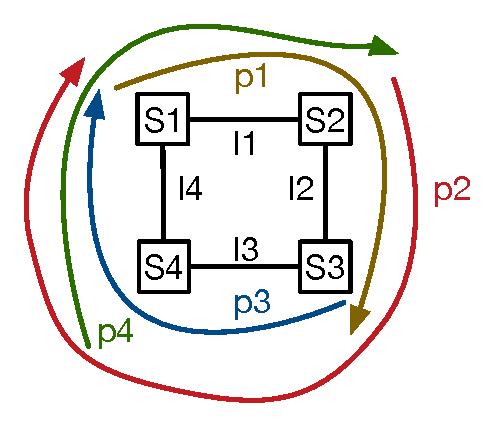
\includegraphics[width=0.35\textwidth] {figs/solution_example1_a}
	}
	
	\subfloat[short for lof][Two optimal CDGs.] {
		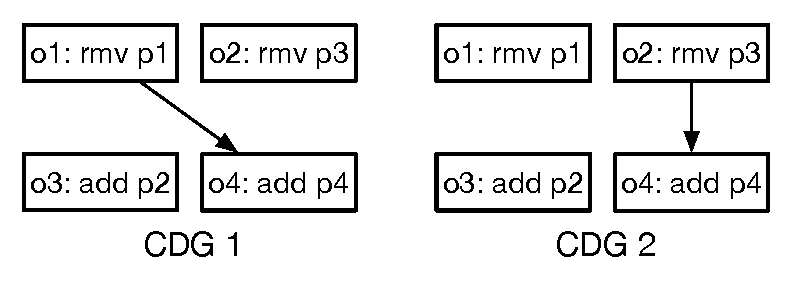
\includegraphics[width=0.45\textwidth] {figs/solution_example1_b}
	}
	
	\caption{An example to illustrate the solution. The network topology is a 4-node cycle. $P_s=\{p1, p3\}$ and $P_t=\{p2, p4\}$. In this example, we assume the time cost to configuring a path is equal to the number of switches this path traverses in the cycle.}\label{fig:solution_example1}
	
\end{figure}

In Fig.~\ref{fig:solution_example1}, we use a simple example to illustrate how our solution works. In this example, $P_s=\{p1, p3\}$ and $P_t=\{p2, p4\}$. As we can see in Fig.~\ref{fig:solution_example1}(a), paths in $P_s \cup P_t$ introduce a cyclic buffer dependency to the network. It is easy to know $P_s^{l1,l2} = \{p1\}$, $P_s^{l3,l4} = \{p3\}$, $P_t^{l2,l3} = \{p2\}$, $P_t^{l3,l4} = \{p2\}$ and $P_t^{l4,l1} = \{p4\}$.

Let $t_{add}(p)$ and $t_{rmv}(p)$ be the time cost to add and remove a path p, respectively. In this example, we assume  the time cost to configuring a path is equal to the number of switches this path traverses in the cycle. So we have $t_{rmv}(p1)=3$, $t_{add}(p2)=4$, $t_{rmv}(p3)=3$ and $t_{add}(p4)=4$.

Our solution will calculate the time cost for all the path sets contributed to some buffer dependency edge. The results are as follows $t(P_s^{l1,l2}) = 3$, $t(P_s^{l3,l4}) = 3$, $t(P_t^{l2,l3}) = 4$, $t(P_t^{l3,l4}) = 4$, $t(P_t^{l4,l1}) = 3$.

Our solution will then calculate the time cost of path configurations for any pair ($P_s^{lx,ly}$, $P_t^{lm,ln}$), and then choose one optimal pair with minimum time cost. In this example, both ($P_s^{l1,l2}$, $P_t^{l4,l1}$) and ($P_s^{l3,l4}$, $P_t^{l4,l1}$) have minimum time cost, so two optimal CDGs can be constructed, as shown in Fig.~\ref{fig:solution_example1}(b). 


%The intuition behind our solution is that \textit{For each possible cycle in the buffer dependency graph, as long as we ensure that one old dependency link is removed before one new dependency link is added, the reconfiguration process is deadlock-free.} 
%
%The idea of our heuristic solution is as follows: First, for each cycle in the buffer dependency graph, we enumerate all the sets of update actions that can exactly add or remove one dependency link from the graph. Then we pick up two minimum action sets A and B, where A can remove one dependency link for a given cycle while B can add an dependency link for the same cycle. The deadlock-free reconfiguration scheme our solution produces will ensure that A is finished before B starts to be configured.

